%----------------------------------------------------------------
%
%  File    :  survey.tex
%
%  Author  :  Keith Andrews, ISDS, TU Graz, Austria
%
%  Created :  24 Mar 2010
%
%  Changed :  04 Mar 2019
%
%----------------------------------------------------------------


\documentclass[11pt,onecolumn,twoside]{report}

\usepackage[
  a4paper,
  twoside,
  top=5mm,                % top margin
  bottom=7mm,             % bottom margin
  inner=20mm,             % inner margin (next to binding)
  outer=20mm,             % outer margin (opposite binding)
  bindingoffset=10mm,     % on binding side
  includeheadfoot,        % include head(er) and foot(er)
  headheight=10mm,        % height of header
  headsep=15mm,           % sep between header and text body
  footskip=15mm,          % sep between body and baseline of footer
  footnotesep = 10mm plus 2mm minus 0mm  % bottom of body to top of footnote
]{geometry}
% A4 paper is w=210m, h=297mm



\newcommand{\fullh}{24cm}         % height of figures for 1 per page
\newcommand{\halfh}{9.5cm}        % height of figures for 2 per page
\newcommand{\thirdh}{6cm}         % height of figures for 3 per page


\setlength{\parindent}{1em}       % less indentation
\setlength{\parskip}{5pt plus 1pt minus 1pt}  % space before a paragraph


% \tolerance is set by LaTeX to 200
% \sloppy sets \tolerance = 9999
% which allows LaTeX more tolerance in adding word spacing

% \sloppy
% \fussy
% \tolerance = 1000

\tolerance=400 
% makes some lines with lots of white space, but      
% tends to prevent words from sticking out in the margin



\setcounter{tocdepth}{3}        % lowest section level entered in ToC
\setcounter{secnumdepth}{3}     % lowest section level still numbered




\usepackage[T1]{fontenc}        % 8-bit output chars (must be before inputenx)
\usepackage[utf8]{inputenx}     % input char encoding

\usepackage[english,austrian,british]{babel}

\usepackage{newtxtext}          % newer times fonts
\usepackage{newtxmath}

\usepackage{relsize}            % relative font sizes \smaller \larger
\usepackage{float}              % H for float placement
\usepackage{setspace}           % line spacing

\usepackage{textcomp}           % symbols such as \texttimes and \texteuro
\usepackage{latexsym}
\usepackage{fontawesome}        % fontawesome symbols

\usepackage{siunitx}            % prettier number formatting
\sisetup{%
  group-separator={,},
}
\usepackage[super]{nth}         % 1st, 2nd, 3rd, etc.

\usepackage{xspace}
\usepackage{xstring}            % string manipulation macros
\usepackage{xparse}             % commands with optional arguments
\usepackage{etoolbox}           % for \newrobustcmd
\usepackage{makecmds}           % for \makecommand
\usepackage{calc}               % for math calculations

\usepackage[svgnames,table,xcdraw]{xcolor}
\definecolor{darkgreen}{rgb}{0.0,0.2,0.0}
\definecolor{darkblue}{rgb}{0.0,0.0,0.2}
\definecolor{darkred}{rgb}{0.2,0.0,0.0}
\definecolor{verylightgrey}{gray}{0.95}
\definecolor{lightgrey}{gray}{0.9}
\definecolor{grey}{gray}{0.7}
\definecolor{black}{gray}{0.0}


\usepackage{longtable}
\usepackage{multirow}
\usepackage{tabularx}

\usepackage{verbdef}            % define robust verb strings
\usepackage{verbatim}
\usepackage{comment}



% better lists
\usepackage{enumitem}

\setlist{
  topsep=0pt,
  partopsep=0pt,
  parsep=0.6ex,
  itemsep=1.2ex,
  left=\parindent .. 2\parindent,    % bullet .. start ot text
}

\setlist[description]{
  style=sameline,
}




\usepackage{listings}                 % for listings of source code

\makeatletter
\newlength{\numwidth}%
\setlength{\numwidth}{\widthof{\normalfont{\lst@numberstyle{99}}}}% Up to 2-digit (99) line numbers
\def\lst@PlaceNumber{%
  \makebox[\numwidth+1em][l]{%
    \makebox[\numwidth][r]{\normalfont\lst@numberstyle{\thelstnumber}}%
  }%
}
\makeatother

% lstset strategy: define defaults here for
% all non-floating listings
% floated listings override these settings later

\lstset{                              % set parameters for listings
  floatplacement=tp,                  % default float placement
  numberbychapter,
  inputencoding=utf8,
  language=,                          % empty = plain text
  basicstyle=\small\ttfamily,
  tabsize=2,
  xleftmargin=2\parindent,
  xrightmargin=2\parindent,
  frame=none,
  framexleftmargin=0mm,
  rulesepcolor=\color{verylightgrey},
  numbers=none,
  numberstyle=\scriptsize,
  numbersep=2ex,
  breaklines,
  showtabs=false,
  showspaces=false,
  showstringspaces=false,
  keywordstyle=\color{black},
  commentstyle=\color{SteelBlue},
  identifierstyle=,
  stringstyle=,
  captionpos=b,
  abovecaptionskip=\abovecaptionskip,
  belowcaptionskip=\belowcaptionskip,
  extendedchars=true,
  literate=%
    {©}{{\textcopyright}}1
    {€}{{\texteuro}}1
    {Ö}{{\"O}}1
    {Ä}{{\"A}}1
    {Ü}{{\"U}}1
    {ß}{{\ss}}1
    {ö}{{\"o}}1
    {ä}{{\"a}}1
    {ü}{{\"u}}1,       % map some utf8 chars for listings
}


\lstdefinelanguage{biblatex}   % based on biblatex v 2.7a from 2013-07-14
{
  keywords={%
    @article,@book,@mvbook,@inbook,@bookinbook,@suppbook,%
    @booklet,@collection,@mvcollection,@incollection,@suppcollection,%
    @manual,@misc,@online,@patent,@periodical,@suppperiodical,%
    @proceedings,@mvproceedings,@inproceedings,@reference,@mvreference,%
    @inreference,@report,@set,@thesis,@unpublished,@xdata,%
    @conference,@electronic,@mastersthesis,@phdthesis,@techreport,@www,%
    @artwork,@audio,@bibnote,@commentary,@image,@jurisdiction,@legislation,%
    @legal,@letter,@movie,@music,@performance,@review,@software,%
    @standard,@video%
  },
  sensitive=false,
  comment=[l][\itshape]{@comment},
  morecomment=[l]{\%},
}

\lstdefinelanguage{CSS}
{
  alsoletter={-},
  morekeywords={%
  color,background,background-color,margin,padding,font,
  font-family,weight,%
  display,position,top,left,right,bottom,list,%
  style,border,size,white,space,min,width%
  },
  sensitive=false,
  morecomment=[l]{//},
  morecomment=[s]{/*}{*/},
  morestring=[b]",
}





\usepackage[compact,nobottomtitles,pagestyles,explicit]{titlesec}
% when using explicit, must explicitly include #1 for titlename

% nobottomtitles
% move section headings close to page bottom to next page
\renewcommand{\bottomtitlespace}{2cm}

% \chaptermark sets the value of \chaptertitle for later
% \@chapapp is defined as \chaptername outside the appendix,
% and as \appendixname within the appendix.
\makeatletter
\titleformat{\chapter}
[display]                                            % shape
{\chaptermark{\thechapter~~#1}\sffamily\bfseries}    % format
{\huge\@chapapp\ \thechapter}                        % label
{4ex}                                                % sep
{\Huge#1}                                            % before-code
\makeatother

\titleformat{name=\chapter,numberless}
[block]                                              % shape
{\chaptermark{#1}\sffamily\bfseries}                 % format
{}                                                   % label
{0ex}                                                % sep
{\Huge#1}                                            % before-code

\titleformat{\section}
{\normalfont\Large\sffamily\bfseries}{\thesection}{0.8em}{#1}

\titleformat{\subsection}
{\normalfont\large\sffamily\bfseries}{\thesubsection}{0.8em}{#1}

\titleformat{\subsubsection}
{\normalfont\normalsize\sffamily\bfseries}{\thesubsubsection}{0.8em}{#1}

\titleformat{\paragraph}[runin]
{\normalfont\normalsize\sffamily\bfseries}{\theparagraph}{0.8em}{#1}

\titleformat{\subparagraph}[runin]
{\normalfont\normalsize\sffamily\bfseries}{\thesubparagraph}{0.8em}{#1}


% vertical spacing before and after section titles
\titlespacing*{\section}
{0pt}{3.5ex plus 0.5ex minus 0.5ex}{0ex plus 0ex minus 0.2ex}

\titlespacing*{\subsection}
{0pt}{2.5ex plus 0.5ex minus 0.5ex}{0ex plus 0ex minus 0.2ex}

\titlespacing*{\subsubsection}
{0pt}{2ex plus 0.5ex minus 0.5ex}{0ex plus 0ex minus 0.2ex}


% define page headings how I want them

\newpagestyle{main}[\small]{
% \addtolength\headheight{6.7pt}
% \headrule
\sethead%
[{\parbox[t]{0.3\textwidth}%                    % even left
  {\sffamily\thepage}}]
[]%                                             % even centre
[{\parbox[t]{0.6\textwidth}%                    % even right
  {\raggedleft\sffamily\chaptertitle}}]
{{\parbox[t]{0.6\textwidth}%                    % odd left
  {\sffamily\sectiontitle}}}%
{}%                                             % odd centre
{{\parbox[t]{0.3\textwidth}%                    % odd right
  {\raggedleft\sffamily\thepage}}}
}



\usepackage{titletoc}

% Add extra per-chapter space to LoL to mimic LoF and LoT
% (requires package etoolbox)
\makeatletter
\patchcmd{\@chapter}% <cmd>
  {\addtocontents}% <search>
  {\addtocontents{lol}{\protect\addvspace{10\p@}}% add per-chapter space
   \addtocontents}% <replace>
  {}{}% <success><failure>
\makeatother

% Configure LoL to mimic LoF and LoT
\contentsuse{lstlisting}{lol}
\titlecontents{lstlisting}
  [3.8em]                      % left indent
  {\addvspace{1.5mm}}          % above-code per entry
  {\contentslabel{2.3em}}      % format for numbered entry
  {\hspace*{-2.3em}}           % format for unnumbered entry
  {\titlerule*[2.7mm]{.} \contentspage}  % dots and page num per entry
  []                           % below-code per entry

\renewcommand{\lstlistlistingname}{List of Listings}





% sensible settings for floats

\setlength{\textfloatsep}{9mm plus 2mm minus 2mm}
\setlength{\floatsep}{9mm plus 2mm minus 2mm}
\setlength{\intextsep}{9mm plus 2mm minus 2mm}

\setlength{\dbltextfloatsep}{9mm plus 2mm minus 2mm}
\setlength{\dblfloatsep}{9mm plus 2mm minus 2mm}

\setlength{\abovecaptionskip}{4mm plus 2mm minus 1mm}
\setlength{\belowcaptionskip}{0mm}

% See http://www-rohan.sdsu.edu/~aty/bibliog/latex/floats.html
% See https://robjhyndman.com/hyndsight/latex-floats/

\setcounter{topnumber}{2}               % max num floats at top of page
\setcounter{dbltopnumber}{2}            % max num floats on 2col page
\setcounter{bottomnumber}{2}            % max num floats at bottom of page
\setcounter{totalnumber}{4}             % max num floats on a page

\renewcommand{\topfraction}{0.8}        % max fraction of floats at top
\renewcommand{\dbltopfraction}{0.9}     % max fraction of floats at top 2col
\renewcommand{\bottomfraction}{0.8}     % max fraction of floats at bottom
\renewcommand{\textfraction}{0.2}       % min fraction of text

% only for entirely float pages:
\renewcommand{\floatpagefraction}{0.7}      % min page fraction having floats
\renewcommand{\dblfloatpagefraction}{0.7}   % min 2col page fraction having floats


% \usepackage[section,above,below]{placeins}  % keep floats to their own section




% use caption and subfig (caption2 and subfigure are now obsolete)

\usepackage[
  position=bottom,
  margin=1cm,
  font=small,
  labelfont={bf,sf},
  format=hang,
  indention=0mm,
]{caption,subfig}

\captionsetup[subfigure]{
  margin=0pt,
  parskip=0pt,
  hangindent=0pt,
  indention=0pt,
  singlelinecheck=true,
  farskip=4mm,            % skip above subfig (assuming captions at bottom)
  captionskip=2mm,        % skip between subfig and subcaption
}


\usepackage[hyphens,obeyspaces]{url}
\def\UrlFont{\smaller\ttfamily}





\usepackage[short]{datetime}   % load datetime *after* babel, requires fmtcount
% \newdateformat{britdate}{%
% \ordinaldate{\THEDAY} \,\monthname[\THEMONTH] \THEYEAR
% }
\newdateformat{unixdate}{%
\twodigit{\THEDAY}~\shortmonthname[\THEMONTH]~\THEYEAR
}



\usepackage[
  autostyle=true,          % adapt quote style to current language
  english=british,         % british english as default
  threshold=1,             % set block quotations >1 line in display mode
  maxlevel=4,              % max nesting level
]{csquotes}

\usepackage[
  indentfirst=false,
  vskip=0pt,               % by default would be \topsep + \partopsep.
]{quoting}

% tell csquotes to use quoting environment
% for \displayquote and \blockquote
\SetBlockEnvironment{quoting}

% if cite is issued by a csquote command
\renewcommand{\mkcitation}[1]{\space#1}

% I prefer double quotes as outer
\DeclareQuoteStyle{keithbritish}%  [variant]{style}
  {\textquotedblleft}%                      opening outer mark
  {\textquotedblright}%                     closing outer mark
  [0.05em]%
  {\textquoteleft}%                         opening inner mark
  {\textquoteright}%                        closing inner mark

\ExecuteQuoteOptions{style=keithbritish}





\usepackage[
  backend=biber,
  style=ext-authoryear,        % defined in biblatex-ext package
  sorting=nyt,
  useprefix,                   % van and von are part of second name
  mergedate=false,             % only for authoryear style
  dashed=false,                % only for authoryear style
  abbreviate=false,
  maxcitenames=2,              % if > 2 authors,
  mincitenames=1,              % use first 1 then et al
  maxbibnames=99,              % if > 99 authors,
  minbibnames=6,               % use first 6 then et al
  uniquelist=minyear,
  uniquename=init,
  hyperref=true,
  backref=true,
  backrefstyle=two,
  sortlocale=en,
]{biblatex}


% set for csquotes, but \autocite only available
% after biblatex is loaded
\SetCiteCommand{\autocite}    % or maybe \parencite

% more space between entries in bib
\setlength\bibitemsep{1.5\itemsep}

% kandrews: replace round brackets with square brackets in citations
\DeclareOuterCiteDelims{parencite}{\bibopenbracket}{\bibclosebracket}
\DeclareInnerCiteDelims{textcite}{\bibopenbracket}{\bibclosebracket}

% kandrews: replace round brackets with square brackets in bibliography
% biblabeldate is a biblatex-ext feature
\DeclareFieldFormat{biblabeldate}{\mkbibbrackets{#1}}


% remove URL: from in front of URLs
\DeclareFieldFormat{url}{\url{#1}}
\DeclareFieldFormat{doi}{\doi{#1}}
\DeclareFieldFormat{isbn}{\isbn{#1}}
\DeclareFieldFormat{issn}{\issn{#1}}

% suppress urldate field
\AtEveryBibitem{\clearfield{urlyear}}

% remove In: from @article and @inproceedings entries
% https://tex.stackexchange.com/questions/10682/suppress-in-biblatex
\renewbibmacro{in:}{%
  \ifboolexpr{%
     test {\ifentrytype{article}}%
     or
     test {\ifentrytype{inproceedings}}%
  }{}{\printtext{\bibstring{in}\intitlepunct}}%
}

% make all entry titles italic
% (also removes quotation marks from around titles)
% https://tex.stackexchange.com/questions/311816/want-title-in-simple-numeric-not-italic-through-bibliography
\DeclareFieldFormat*{title}{\mkbibitalic{#1}}
\DeclareFieldFormat*{citetitle}{\mkbibitalic{#1}}

% make journal names non-italic
\DeclareFieldFormat{journaltitle}{#1\isdot}

% make proceedings names non-italic
\DeclareFieldFormat[inproceedings]{booktitle}{#1\isdot}

% use nth for edition
\DeclareFieldFormat{edition}{%
  \ifinteger{#1}
    {\nth{#1}~\bibstring{edition}}
    {#1\isdot}}

% overwrite some standard strings in english.lbx
\DefineBibliographyStrings{english}{%
  edition          = {Edition},
  mathesis         = {Master's Thesis},
  phdthesis        = {PhD\addabbrvspace Thesis},
}


% kandrews
% use Unix format for dates in biblio:
% 29 Dec 2015, 01 Oct 2018, etc.

% for now, define under lang english not british
% due to bug in biblatex 3.11

\DefineBibliographyStrings{english}{%
  january          = {Jan},
  february         = {Feb},
  march            = {Mar},
  april            = {Apr},
  may              = {May},
  june             = {Jun},
  july             = {Jul},
  august           = {Aug},
  september        = {Sep},
  october          = {Oct},
  november         = {Nov},
  december         = {Dec},
}

\DefineBibliographyExtras{english}{%
% #1 = year, #2 = month, #3 = day
\protected\def\mkbibdatelong#1#2#3{%
  \iffieldundef{#3}
    {}
    {\mkdayzeros{\thefield{#3}}%
     \iffieldundef{#2}{}{\nobreakspace}}%
  \iffieldundef{#2}
    {}
    {\mkbibmonth{\thefield{#2}}%
     \iffieldundef{#1}{}{\space}}%
  \iffieldbibstring{#1}{\bibstring{\thefield{#1}}}{\mkyearzeros{\thefield{#1}}}}%
%
\protected\def\mkbibdateshort#1#2#3{%
  \iffieldundef{#3}
    {}
    {\mkdayzeros{\thefield{#3}}%
     \iffieldundef{#2}{}{\nobreakspace}}%
  \iffieldundef{#2}
    {}
    {\mkbibmonth{\thefield{#2}}%
     \iffieldundef{#1}{}{\space}}%
  \iffieldbibstring{#1}{\bibstring{\thefield{#1}}}{\mkyearzeros{\thefield{#1}}}}%
}


% patch for biblatex 3.11 issue with babel .lbx files
% https://github.com/plk/biblatex/issues/742
% should no longer be necessary with biblatex 3.12
\makeatletter
\protected\long\def\blx@lbx@input@handler@simple#1#2#3#4#5#6{%
  \blx@info@noline{Trying to load #2..}%
  \IfFileExists{#1}
    {\blx@info@noline{... file '#1' found}%
     #3\@@input\@filef@und#4#5%
     \ifcsundef{blx@file@lbx@simple@#1}
       {\listxadd\blx@list@req@stat{#1}%
        \@addtofilelist{#1}%
        \global\cslet{blx@file@lbx@simple@#1}\@empty}
       {}}
    {\blx@info@noline{... file '#1' not found}#6}}

\protected\long\def\blx@lbx@input@handler@once#1#2#3#4#5#6{%
  \ifcsundef{blx@file@lbx@once@#1}
    {\blx@info@noline{Trying to load #2..}%
     \IfFileExists{#1}
       {\blx@info@noline{... file '#1' found}%
        #3\@@input\@filef@und#4#5%
        \ifcsundef{blx@file@lbx@simple@#1}
          {\listxadd\blx@list@req@stat{#1}%
           \@addtofilelist{#1}}
          {}}
       {\blx@info@noline{... file '#1' not found}#6}%
     \global\cslet{blx@file@lbx@once@#1}\@empty
     \global\cslet{blx@file@lbx@simple@#1}\@empty}
    {#5}}
\makeatother




\addbibresource{links.bib}





% adapt pdftitle, pdfsubject, pdfauthor, pdfkeywords
% for your survey paper

\usepackage{ifpdf}

\ifpdf
  % pdflatex
  \usepackage[pdftex]{graphicx}
  \DeclareGraphicsExtensions{.pdf,.jpg,.png}
  \pdfcompresslevel=9
  \pdfpageheight=297mm
  \pdfpagewidth=210mm
  \usepackage[         % hyperref should be last package loaded
    unicode,
    pdftex,
    pdfversion=1.7,
    pdftitle={Writing a Survey Paper},
    pdfsubject={Survey Paper Template},
    pdfauthor={Keith Andrews},
    pdfkeywords={survey paper, skeleton, guidelines, template},
    bookmarks,
    bookmarksnumbered,
    linktocpage,
    colorlinks,
    linkcolor=darkred,
    anchorcolor=red,
    citecolor=darkgreen,
    urlcolor=darkblue,
    pdfview={Fit},
    pdfstartview={Fit},
    pdfpagemode=UseOutlines,       % open bookmarks in Acrobat
    plainpages=false,              % avoids duplicate page number problem
    pdfpagelabels,                 % avoids duplicate page number problem
    breaklinks=true,               % allow links exceeding a single line
  ]{hyperref}

\else
  % latex
  \usepackage[dvips]{graphicx}
  \usepackage[dvips]{hyperref}
  \DeclareGraphicsExtensions{.eps}
\fi



% subset of macros from thesis-macros

% \liintro list item intro is a style used when list items have an
% introduction phrase (say in italics) followed by a colon.
\newcommand{\liintro}[1]{\emph{#1}}

% short notes in square brackets
\newcommand{\shortnote}[1]
{%
{{\smaller{}[#1]}}
}


\newcommand{\TODO}[1]
{
{\textcolor{red}{[TODO: #1]}}
}



\newcommand{\imgcredit}[1]
{\smaller{}[#1]}



\newcommand{\copyrightACM}
{%
Copyright \copyright\ by the Association for Computing Machinery, Inc.%
}




\newcommand{\daymonthyear}[3]
{%
\twodigit{#1}\hspace{0.7ex}\nolinebreak[2]\shortmonthname[#2]\hspace{0.7ex}\nolinebreak[2]#3%
}


\newcommand{\monthyear}[2]
{%
\shortmonthname[#1]\hspace{0.7ex}\nolinebreak[2]#2%
}


\newcommand{\yearmonthday}[3]
{%
\twodigit{#3}\hspace{0.7ex}\nolinebreak[2]\shortmonthname[#2]\hspace{0.7ex}\nolinebreak[2]#1%
}


\newcommand{\yearmonth}[2]
{%
\shortmonthname[#2]\hspace{0.7ex}\nolinebreak[2]#1%
}



% link to Amazon or
% http://worldcatlibraries.org/wcpa/isbn/[ISBN number]
% http://amazon.com/exec/obidos/ASIN/#1/keithandrewshcic
% http://amazon.com/dp/#1/

\newrobustcmd{\isbn}[1]
{%
{%
\ifpdf
{\smaller ISBN
\href{http://amazon.co.uk/dp/#1/}{#1}}%
\else
{\smaller ISBN #1}%
\fi
}%
}



% ISSN
% http://www.bl.uk/services/bibliographic/issn.html
% 8 digits, should be printed xxxx-xxxx
% e.g. 0020-0190 is Information Processing Letters, Elsevier
%
% Lookup services:
% http://kmittlib.lib.kmutt.ac.th:81/search/i?SEARCH=0020-0190
% http://worldcatlibraries.org/wcpa/issn/0020-0190

\newrobustcmd{\issn}[1]
{%
{%
\ifpdf
{\smaller ISSN
\href{http://worldcatlibraries.org/wcpa/issn/#1}{#1}}%
\else
{\smaller ISSN #1}%
\fi
}%
}



% DOIs  http://doi.org/  e.g.
% doi:10.1038/nature723
% http://doi.org/10.1038/nature723

\newrobustcmd{\doi}[1]
{%
{%
\def\UrlFont{\smaller\rmfamily}
\ifpdf                                   % pdflatex
\href{http://doi.org/#1}{doi:\protect\nolinkurl{#1}}%
\else                                    % latex
doi:\protect\nolinkurl{#1}%
\fi
}%
}





\newrobustcmd{\website}[1]
{%
\ifpdf                                  % pdflatex
\href{http://#1/}{\nolinkurl{#1}}%
\else                                   % latex
\nolinkurl{#1}%
\fi
}




\newcommand{\news}[1]
{%
\ifpdf
\href{news:#1}{\nolinkurl{#1}}
\else
\nolinkurl{#1}%
\fi
}








% based on url package
% define styles for class, file, and variable names
% which break nicely at line breaks

% make the macros robust so they work inside captions, etc

\newcommand{\ttname}{\begingroup \smaller\urlstyle{tt}\Url}
\newcommand{\rmname}{\begingroup \smaller\urlstyle{rm}\Url}
\newcommand{\sfname}{\begingroup \smaller\urlstyle{sf}\Url}


% fname is for file names and directory names
\newrobustcmd{\fname}[1]{\ttname{#1}}

% vname is for variable names, domain names, email addresses
\newrobustcmd{\vname}[1]{\ttname{#1}}




% for class names, define our own url style

\makeatletter  % protect @ names

% \url@letstyle: New URL style to premit break at any letters.
% Based on \url@ttstyle

\def\Url@letdo{% style assignments for tt fonts or T1 encoding
\def\UrlBreaks{\do\a\do\b\do\c\do\d\do\e\do\f\do\g\do\h\do\i\do\j\do\k\do\l%
               \do\m\do\n\do\o\do\p\do\q\do\r\do\s\do\t\do\u\do\v\do\w\do\x%
               \do\y\do\z%
               \do\A\do\B\do\C\do\D\do\E\do\F\do\G\do\H\do\I\do\J\do\K\do\L%
               \do\M\do\N\do\O\do\P\do\Q\do\R\do\S\do\T\do\U\do\V\do\W\do\X%
               \do\Y\do\Z%
}%
\def\UrlBigBreaks{\do\.\do\@\do\\\do\/\do\!\do\_\do\|\do\%\do\;\do\>\do\]%
 \do\)\do\,\do\?\do\'\do\+\do\=\do\#\do\:\do@url@hyp}%
\def\UrlNoBreaks{\do\(\do\[\do\{\do\<}% (unnecessary)
\def\UrlSpecials{\do\ {\ }}%
\def\UrlOrds{\do\*\do\-\do\~}% any ordinary characters that aren't usually
\Urlmuskip = 0mu plus 1mu%
}

\def\url@letstyle{%
\@ifundefined{selectfont}{\def\UrlFont{\sf}}{\def\UrlFont{\sffamily}}\Url@letdo
}

\makeatother  % unprotect @ names

% class names
\newcommand\letname{\begingroup \smaller\urlstyle{let}\Url}

\newrobustcmd{\cname}[1]{\letname{#1}}






% Euro symbol
\newcommand{\euro}{\texteuro\,}

% times symbol
\newcommand{\timessym}{\texttimes\,}

% approx symbol
\newcommand{\approxsym}{\ensuremath\approx\,}

% plusminus symbol
\newcommand{\plusminussym}{\textpm\,}

% not equal symbol
\newcommand{\neqsym}{\ensuremath{\neq\,}}

% rightarrow symbol
\newcommand{\rightarrowsym}{\ensuremath\rightarrow\,\,}


% thumbs up and thumbs down symbols

\newcommand{\uthumb}{\smaller[2]\raisebox{1pt}{\textcolor{DarkGreen}{\faThumbsUp}}}

\newcommand{\dthumb}{\smaller[2]\raisebox{1pt}{\textcolor{DarkRed}{\faThumbsDown}}}







\begin{document}

\unixdate

\normalsize
\pagestyle{empty}         % for preliminary pages (no numbers shown)
\pagenumbering{Roman}     % for pdf labels




\begin{titlepage}

\begin{center}
\begin{spacing}{1.1}
\Large\sffamily\bfseries
Card Sorting Tools
\end{spacing}

\vspace{1cm}

{\large\sffamily Christopher Oser, Markus Ruplitsch \& Markus Stradner}

\vspace{5mm}

{\large\sffamily Group 3}

\vspace{1cm}

{\large
 706.041 Information Architecture and Web Usability WS 2020/21 \\
 Graz University of Technology \\[1cm]
}

\vspace{1cm}

{25 Nov 2020}

\end{center}



\vspace{2cm}

\begin{quote}
\begin{center}
{\large\sffamily\bfseries Abstract}
\end{center}
TODO
\end{quote}

\vfill

\begin{center}
{\footnotesize\sffamily \copyright ~ Copyright 2020 by the author(s),
except as otherwise noted.}

\vspace{2mm}
{\footnotesize\sffamily This work is placed under a
Creative Commons Attribution 4.0 International
(\href{https://creativecommons.org/licenses/by/4.0/}{CC BY 4.0}) licence.}
\end{center}

\end{titlepage}




\cleardoublepage
\pagestyle{plain}             % for preliminary pages
\pagenumbering{roman}         % for preliminary pages


\begin{spacing}{0.8}
\tableofcontents
\end{spacing}
\addcontentsline{toc}{chapter}{Contents}

\cleardoublepage
\begin{spacing}{0.8}
\listoffigures
\end{spacing}
\addcontentsline{toc}{chapter}{List of Figures}

\cleardoublepage
\begin{spacing}{0.8}
\listoftables
\end{spacing}
\addcontentsline{toc}{chapter}{List of Tables}

\cleardoublepage
\begin{spacing}{0.8}
\renewcommand{\lstlistlistingname}{List of Listings}
\lstlistoflistings
\end{spacing}
\addcontentsline{toc}{chapter}{List of Listings}



\cleardoublepage
\pagestyle{main}              % for main pages
\pagenumbering{arabic}        % for main pages


\cleardoublepage
\chapter{Introduction}

\label{chap:Intro}

This chapter explains the differences between open, closed and hybrid card
sorting and the different challenges that come with each method. Furthermore, 
this chapter will also include an overview of all the reviewed tools as well as 
a detailed description of our review process and which features we focused on.


\section{Card Sorting}

Card sorting is a type of usability test in which participants are
asked to sort cards into different categories. Usually a distinction
is made between open, closed, and hybrid card sorting. Open card
sorting does not provide any predefined categories, and instead users
create their own categories. Closed card sorting gives the
participants a predefined list of categories into which the cards have
to be sorted. Hybrid card sorting is a mix of the two previous models,
where some categories are predefined, but users can create more. This
survey focuses on the capabilities of tools to work with open card
sorting studies.

Open card sorting comes with some additional challenges, since the
number of categories created by participants is not limited, and in
some instances sub-categories may be permitted. Furthermore, many of
the categories defined by users will be extremely similar or the same,
but may use different words to describe the same thing. These
categories then have to be merged in an additional step before drawing
any meaningful conclusions.

In case the reader is interested in learning more about card sorting, the book
Card Sorting: Designing Usable Categories by Donna
\textcite{DonnaSpencer1} is strongly recommended. Alternatively, Card sorting: a 
definitive guide by Donna \textcite{DonnaSpencer2} provides a shorter overview of how 
card sorting works and its benefits.


\section{Tools}

This chapter lists the tools in the card sorting field that were
reviewed in the process of this survey. These tools can be further
grouped by their functionalities. One tool, kardSort, is only intended
for the card sorting and offers no analytics at all. Some other tools
are only able to analyze previous card sort experiments, but offer no
sorting capabilities. Finally the remaining tools offer both sorting
and analytic capabilities. An overview can be seen in
Table~\ref{tab:reviewed-tools}.

\begin{table}[tp]
\centering
\begin{tabularx}
{\linewidth}{|X|X|X|}
\hline \textbf{Card Sorting} & \textbf{Analytics} & \textbf{Both}\\ 
\hline kardSort & SynCaps v3 & UXtweak \\ 
\hline & Casolysis & ProvenByUsers \\
\hline & CSA & xSort \\
\hline & & OptimalSort \\
\hline
\end{tabularx} 
\caption[Reviewed Tools] 
{ 
This table summarizes all the tools that were reviewed and categorizes
them by functionality.
}
\label{tab:reviewed-tools}
\end{table}


More tools were previewed before coming to a decision as to which
tools will be in the final survey. There were tools we were not able
to review as they are no longer available or have been acquired by
competitors. One tool, ~\textcite{UserZoom}, offers no free version
and did not answer to our inquiry for a review version. We listed all
tools that we looked at but did not review below:

\begin{itemize}
    \item ~\parencite{SortIt} (not buildable)
    \item ~\parencite{UserZoom} (did not respond to inquiry)
    \item UsabilityTools UXSuite (acquired by competitor)
    \item ~\parencite{SimpleCardSort} (discontinued)
    \item ~\parencite{usabiliTEST} (acquired by competitor)
    \item ConceptCodify (acquired by competitor)
\end{itemize}


\section{Review Process} The reviewing of tools was done in parallel
by three different  reviewers. In order to ensure streamlined reviews
and produce comparable results a review process was defined. Each
reviewer had to perform the same tasks and check for certain
pre-defined features. These features are listed below:

\begin{itemize}
    \item Participant limit
    \item Card limit
    \item Business model
    \item Availability of documentation
    \item Support for sub-categories
    \item Possibility for questionnaires
    \item Import data capabilities
    \item Export data capabilities
    \item User session playbacks
    \item Data preparation capabilities
    \item Types of analytical visualizations
\end{itemize}

Once a review had taken place. It was discussed
in a meeting with the other reviewers and ratings were assigned in
accordance with all members.

Each tool was tested with 2 datasets made up of two sets of cards. One
dataset is made up of 10 animals and the second is a list of 55 car
manufacturers. The cards were then used in open card sorting
experiments by the reviewers. The datasets can be viewed in Table
~\ref{tab:dataset-animal} and ~\ref{tab:dataset-car}.

\begin{table}[tp]
\centering
\begin{tabularx}
{\linewidth}{|X|X|X|X|X|}
\hline
Dog& Elephant  & Whale     & Lion& Mouse         \\
\hline
Cow       & Bear& Butterfly & Snake  & Badger    \\
\hline
\end{tabularx} 
\caption[Animal Dataset] 
{ 
This table lists all the cards in the animal dataset.
}
\label{tab:dataset-animal}
\end{table}

\begin{table}[bp]
\centering
\begin{tabularx}
{\linewidth}{|X|X|X|X|X|}
\hline
Volkswagen    & BYD      & Ford         & Infiniti    & Rimac   \\
\hline
Kia           & Skoda    & Cadillac     & Mitsubishi  & Jeep    \\
\hline
Honda         & Bugatti  & Jaguar       & Dodge       & Lincoln \\
\hline
Toyota        & Citroen  & Aston Martin & GMC         & Smart   \\
\hline
Porsche       & Hyundai  & Chrystler    & Lexus       & Tesla   \\
\hline
Seat          & Nissan   & Subaru       & Range Rover & Lancia  \\
\hline
Mazda         & Saab     & Lamborghini  & Rolls-Royce & Dacia   \\
\hline
BMW           & Renault  & Koenigsegg   & Volvo       & Lotus   \\
\hline
Audi          & Peugeot  & Alfa Romeo   & Suzuki      & Mini    \\
\hline
KTM           & Ferrari  & Fiat         & Bentley     & Lada    \\
\hline
Mercedes-Benz & Chevrolet& Maserati     & McLaren     &        \\
\hline
\end{tabularx} 
\caption[Car Dataset] 
{ 
This table lists all the cards in the car manufacturer dataset.
}
\label{tab:dataset-car}
\end{table}



\cleardoublepage
\chapter{TOOL}

\label{chap:tool}


TOOL INTRODUCTION.


\section{Business Model}

\section{Card Sorting}

\section{Analytics}

\section{Summary \& Ratings}

\cleardoublepage
\chapter{TOOL}

\label{chap:tool}


TOOL INTRODUCTION.


\section{Business Model}

\section{Card Sorting}

\section{Analytics}

\section{Summary \& Ratings}

\cleardoublepage
\chapter{TOOL}

\label{chap:tool}


TOOL INTRODUCTION.


\section{Business Model}

\section{Card Sorting}

\section{Analytics}

\section{Summary \& Ratings}

\cleardoublepage
\chapter{TOOL}

\label{chap:tool}


TOOL INTRODUCTION.


\section{Business Model}

\section{Card Sorting}

\section{Analytics}

\section{Summary \& Ratings}

\cleardoublepage
\chapter{kardSort}

\label{chap:kardSort}


kardSort is an online card sorting tool that was created by a single
developer as their master's thesis. It is a very intuitive and simple
tool that is easy and rewarding to use. That being said it does lack
in some features in comparison to its peers and might be a little too
simple for some users~\parencite{kardSort}.

\begin{figure}[tp] 
\centering
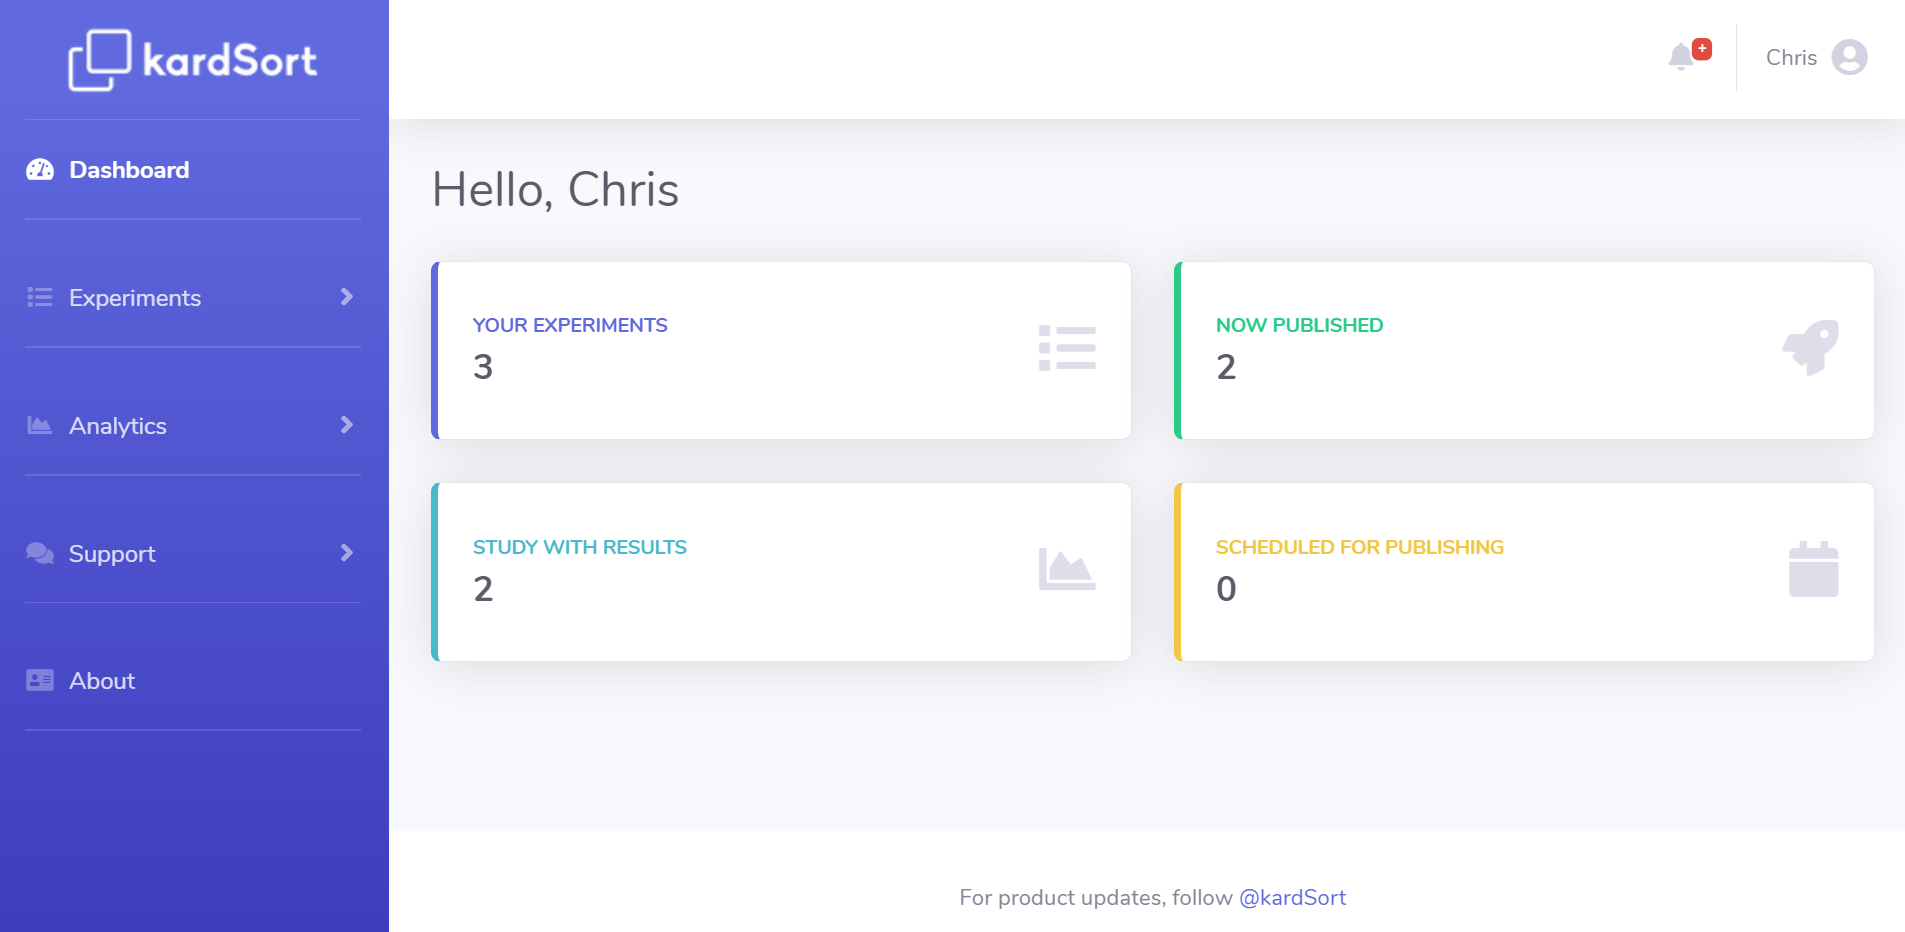
\includegraphics[keepaspectratio,width=\linewidth,height=\halfh]{images/kardsort-dashboard.png}
\caption[kardSort Application] { This is the base view in kardSort.
It shows you an overview of your experiments and in the side menu all
further actions can be performed.
\imgcredit{Screenshot was captured by Christopher Oser using
\textcite{kardSort} on Google Chrome 84.} }
\label{fig:kardSort1}
\end{figure}


\section{Business Model}
As to be expected from a master's thesis project the tool is fully 
free of charge. All features are accessible immediately and there are
no extra features hidden behind some paywall.

The only prerequisite for using the tool is to create an account,
either explicitly for the site or using an existing Google account.
The account make sure all the work within the tool is saved and can be
accessed again even after the session has been terminated. This also
enables access to the experiments, regardless of device or geo-
location. All experiments and data are saved in a cloud that is
provided by kardSort.

\section{Card Sorting}
The card sorting in kardSort is very straight forward. There are no 
special gimmicks or features that make it stand out from other tools.
They offer open, closed and hybrid card sorting. It is possible to
include a welcome message and instructions for every experiment.

A feature that is quite handy at times, is the possibility to include
a customizable questionnaire for an experiment. This questionnaire can
be made up of any number of single line text, multi line text,
check box or radio button questions and is displayed right before the
actual sorting.

In terms of limitations during card sorting, we were able to find two.
Firstly it is not possible to perform an experiment with more than 50
cards. This is a hard limit set during development that offers no
workaround by a user. If this is a deal-breaking limitation, it could
be possible to contact the developer about it and request more cards
per experiment, as the tool does have a feature request page.
Secondly it is quite exhausting working with more than five
categories, as the way the tool is defined, it adds new categories at
the very right of the previous categories. Therefore a lot of
horizontal scrolling is involved when browsing larger number of
categories.

A detailed summary of features can be viewed in
Table~\ref{tab:features-kardSort}.

\begin{figure}[tp] 
\centering
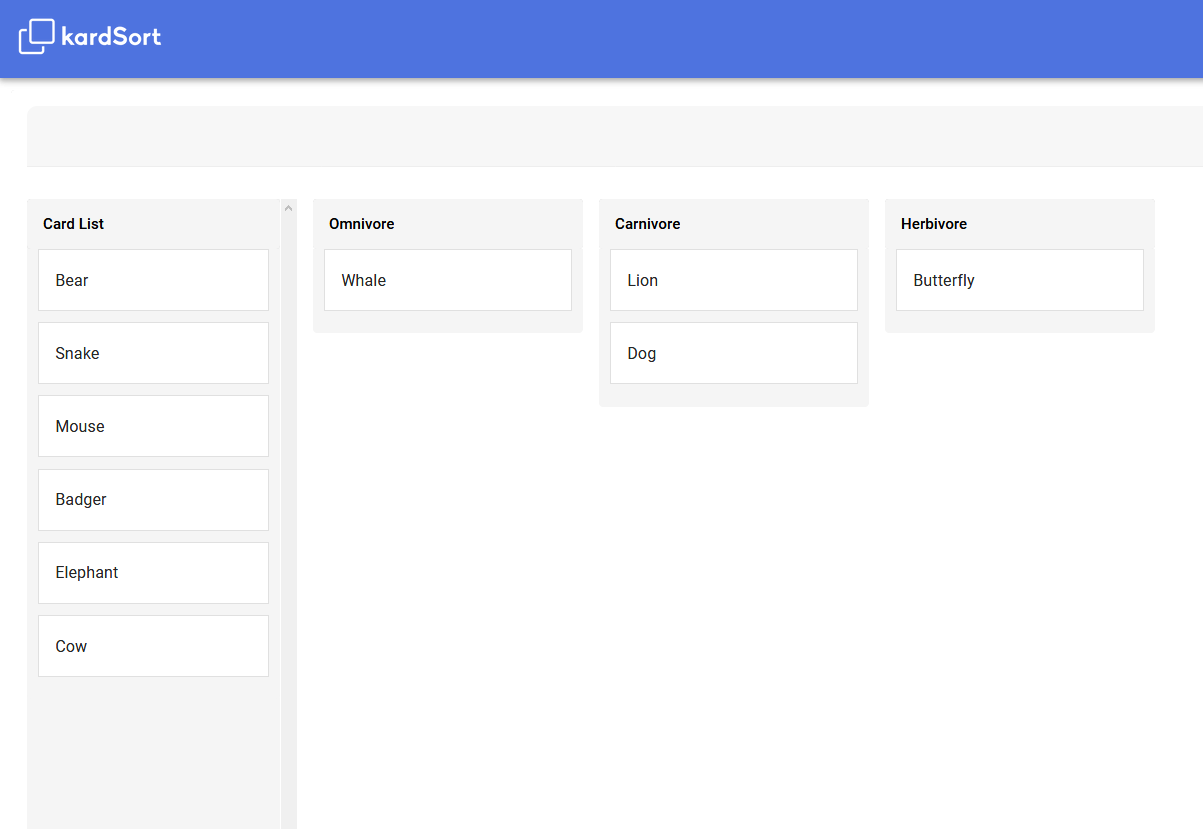
\includegraphics[keepaspectratio,width=\linewidth,height=\halfh]{images/kardsort-sorting.png}
\caption[kardSort Card Sorting] { This is a screenshot during the card
sorting process in kardSort.
\imgcredit{Screenshot was captured by Christopher Oser using
\textcite{kardSort} on Google Chrome 84.} }
\label{fig:kardSort2}
\end{figure}


\section{Analytics} This is the caveat of kardSort, the part where it
is truly lacking, because it does not offer any type of analytics for
its experiments. There is the  possibility of exporting all the
relevant data of an experiment to .csv files for manual analytics or
data preparation. 

Additionally it also offers to export experiment data in the required
format of two other card sorting analytics tools, namely Casolysis and
SynCaps. These two tools are both free of charge and provide good
analytics for card sorting experiments. Further information about them
can be found in the respective Chapters~\ref{chap:SynCaps} and
\TODO{add chapter} within this survey.

\begin{table}[tp]
\centering
\begin{tabularx}
{\linewidth}{|l|X|}
\hline \textbf{Feature/Characteristic} & \textbf{Availability in kardSort} \\ 
\hline Card Sorting & Open, closed and hybrid. \\ 
\hline Card Limit & 50 \\
\hline Participant Limit & None. \\
\hline Analytics & Only export for Casolysis and SynCaps. No in-tool
analytics \\ 
\hline Documentation & None, but tool explains itself very well. No 
documentation was needed during review. \\
\hline Business Model & Free. \\
\hline Import formats & None. All data needs to be entered by hand.\\ 
\hline Export formats & .csv for everything plus formats matching
Casolysis and SynCaps. \\ 
\hline Sub-Categories & No. \\ 
\hline Playback of user-sessions & No. \\ 
\hline Data preparation & Only by hand through export files. \\ 
\hline
\end{tabularx} 
\caption[Feature summary of kardSort] 
{ 
This table summarizes all the features and characteristics of kardSort
to provide an easy to read overview.
}
\label{tab:features-kardSort}
\end{table}


\section{Summary \& Ratings}
All in all kardSort provides a very good card sorting experience. 
Everything it does it does well. Apart from a card limit and some 
formatting with the categories there were no issues when reviewing 
the tool.

Of course it lacks greatly in comparison to other tools, since it 
does not provide any own analytics. Although it does provide you
with the option to do the analytics elsewhere. So this could be a
possible compromise for some users, making this nonetheless a viable
option when in search for a card sorting tool.

For a quick overview and to make it easier to compare to other tools
in this paper, we agreed on 4 ratings for the tool. The ratings can be
found in Table~\ref{tab:rating-kardSort} and range from 0-5.

\begin{table}[tp] 
\centering 
\begin{tabularx}{\linewidth}{|X|X|X|X|X|}
\hline
Simplicity & Documentation & Features & Business Model & Average \\ 
\hline 
5 & 1 & 1 & 5 & 3.0 \\ 
\hline 
\end{tabularx} 
\caption[Ratings for kardSort] {
Ratings for kardSort including the average rating.
} 
\label{tab:rating-kardSort}
\end{table}

\cleardoublepage
\chapter{SynCaps}

\label{chap:SynCaps}

SynCaps is an older card sorting tool that is not available online. It
is only usable as an offline Windows program that needs to be 
installed locally. Since 2018 the full package is offered free of 
charge and can be downloaded. It is not trivial to use and requires 
some time spent with the provided documentation videos. Its workflow
is dated and requires some getting used to~\parencite{SynCaps}.

As the tool does not offer any card sorting capabilities, this needs
to be taken care of in some other way. Originally SynCaps was intended
to be used in cooperation with paper card sorting. After the
experiment was done one can import the data into SynCaps and analyze
it. Nowadays it is also very easy to use other card sorting tools and
then import the data into SynCaps for analytics. Figure~\ref{fig:SynCaps1}
gives an overview of what the basic view in the tool looks like.

\begin{figure}[tp] 
\centering
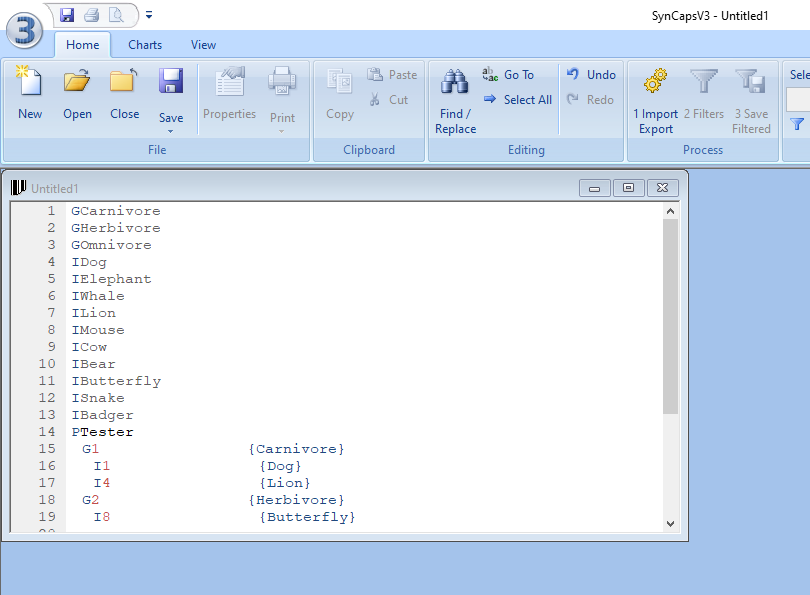
\includegraphics[keepaspectratio,width=\linewidth,height=\halfh]{images/syncaps-sorting.png}
\caption[SynCaps Application] { This is the base view within SynCaps.
All input data is handled within a .txt file as shown in the screenshot.
\imgcredit{Screenshot was captured by Christopher Oser using
\textcite{SynCaps}.} }
\label{fig:SynCaps1}
\end{figure}

\section{Business Model}
As mentioned earlier SynCaps is totally free of charge. There are no
additional features to be unlocked by a paywall. Previously other 
restrictions applied, but since 2018 the tool is not only free of
charge, but also licensing free.

Being an offline program, there is also no need for an account. Any 
data is saved locally and needs to be manually moved to be accessed in
other environments.

\section{Card Sorting}
SynCaps does not provide any card sorting capabilities. It is intended
to be used with paper card sorting or other tools. For paper card
sorting, it provides an option to assign barcodes to cards, for easier
importing of the results after the experiment.

\section{Analytics}
This is were this tool shines. When analyzing results from card
sorting experiments, the options are quite numerous, not so say
overwhelming. Before any analytics, there is the possibility for
data preparation. Users can be singled out, cards as well as categories
can be merged and lots more.

Once the data has been prepared the results can be analyzed within 5
different charts that can be further customized. These charts are made
up of clusterings and dendrograms with different inputs. These charts
are somewhat interactive, as a click on a datapoint will reveal more
information about it, but that is also where the interactivity ends.

The features are summarized in Table~\ref{tab:features-SynCaps}. Furthermore
two analytical visualizations, a clustering and a dendrogram, can be seen
in Figures~\ref{fig:SynCaps2} and \ref{fig:SynCaps3} respectively.

\begin{figure}[tp] 
\centering
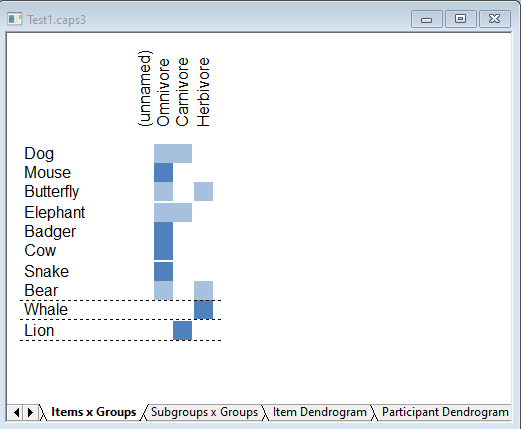
\includegraphics[keepaspectratio,width=\linewidth,height=\halfh]{images/syncaps-diagram-1.png}
\caption[SynCaps Clustering] { This screenshot shows a Cards x Groups
visualization used for analytics.
\imgcredit{Screenshot was captured by Christopher Oser using
\textcite{SynCaps}.} }
\label{fig:SynCaps2}
\end{figure}

\begin{figure}[tp] 
\centering
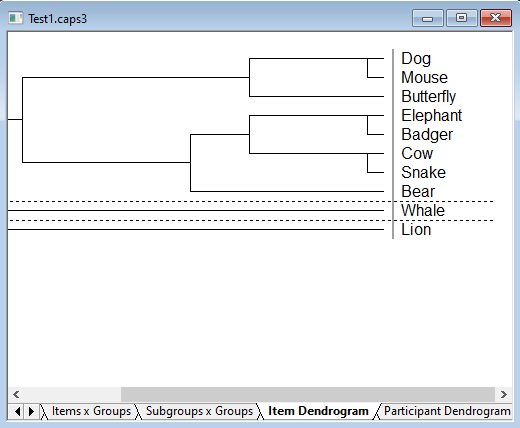
\includegraphics[keepaspectratio,width=\linewidth,height=\halfh]{images/syncaps-diagram-2.png}
\caption[SynCaps Dendrogram] { This screenshot shows a Cards 
dendrogram used for analytics.
\imgcredit{Screenshot was captured by Christopher Oser using
\textcite{SynCaps}.} }
\label{fig:SynCaps3}
\end{figure}

\begin{table}[tp]
\centering
\begin{tabularx}
{\linewidth}{|l|X|}
\hline \textbf{Feature/Characteristic} & \textbf{Availability in SynCaps} \\ 
\hline Card Sorting & None. Paper Cards or other tools needed. \\ 
\hline Card Limit & None. \\
\hline Participant Limit & None. \\
\hline Analytics & Analytics in 5 semi-interactive
charts made up of clusterings and dendrograms \\ 
\hline Documentation & Some dated videos. \\
\hline Business Model & Free. \\
\hline Import formats & .csv, .txt or paste\\ 
\hline Export formats & .csv \\ 
\hline Sub-Categories & Yes, sub-categories are supported \\ 
\hline Playback of user-sessions & No. \\ 
\hline Data preparation & Extensive options from user exclusion to
card merging. \\ 
\hline
\end{tabularx} 
\caption[Feature summary of SynCaps] 
{ 
This table summarizes all the features and characteristics of SynCaps
to provide an easy to read overview.
}
\label{tab:features-SynCaps}
\end{table}


\section{Summary \& Ratings} SynCaps is a solid analytics tool if you
can get past its workflow and learning curve. The videos offered as
documentation, but are not fun to watch to say the least. It offers
many data preparation options and enables efficient evaluation of
results with its many semi-interactive  visualizations.

It is always necessary to pair SynCaps with either physical paper card
sorting or another tool to perform the actual card sorting. If this is
an option, then SynCaps can be very handy for analyzing.

For a quick overview and to make it easier to compare to other tools
in this paper, four ratings were agreed upon to represent the tool. The ratings can be
found in Table~\ref{tab:rating-SynCaps} and range from 0-5.

\begin{table}[tp] 
\centering 
\begin{tabularx}{\linewidth}{|X|X|X|X|X|}
\hline
Simplicity & Documentation & Features & Business Model & Average \\ 
\hline 
1 & 2 & 4 & 5 & 3.0 \\ 
\hline 
\end{tabularx} 
\caption[Ratings for SynCaps] {
Ratings for SynCaps including the average rating.
} 
\label{tab:rating-SynCaps}
\end{table}

\cleardoublepage
\chapter{Casolysis}

\label{chap:Casolysis}

Casolysis is a free card sorting tool that was developed by multiple
students at the University of Paderborn~\parencite{Casolysis}. It is
standalone Windows .exe file that requires no installation. The tool 
is no longer under development, but can still be downloaded from the 
university's website.

Similar to \textcite{SynCaps}  offers no actual card sorting tool, but rather
takes over the analytical part of the process. Card sorting needs to
be done in some other form, be it physical or with a different tool,
and then the results can be imported to Casolysis. Figure~\ref{fig:Casolysis1}
shows the basic view within the tool.

\begin{figure}[tp] 
\centering
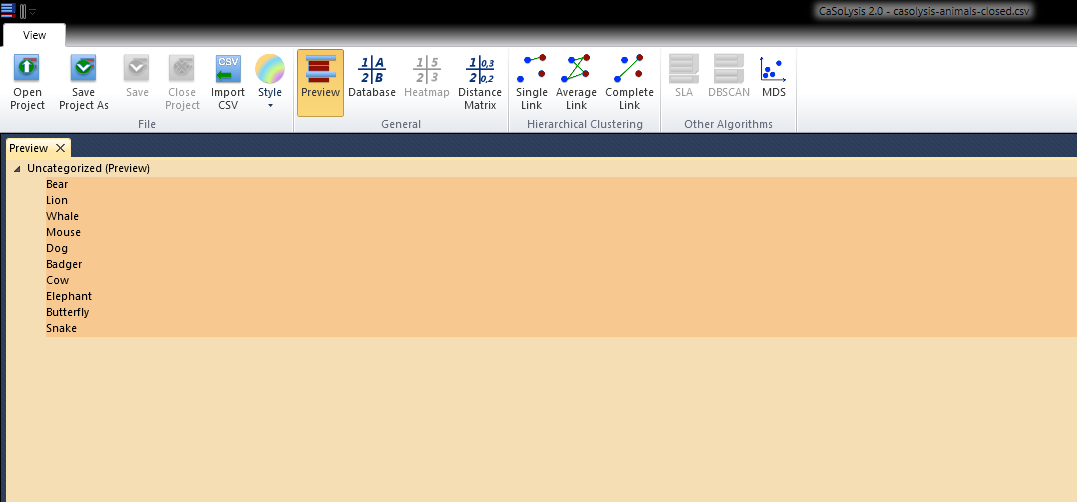
\includegraphics[keepaspectratio,width=\linewidth,height=\halfh]{images/casolysis-sorting.png}
\caption[Casolysis Application] { This is the base view within Casolysis
once data is imported with a .csv file.
\imgcredit{Screenshot was captured by Christopher Oser using
\textcite{Casolysis}.} }
\label{fig:Casolysis1}
\end{figure}

\section{Business Model}
Casolysis is free of charge and can be downloaded an unlimited amount
of times. Its development has seized, but the tool can still be used
in its current form.

Additionally no account is needed to access Casolysis. It does
not even require installation, but can be run straight out of the .exe
file.

\section{Card Sorting}
Casolysis does not support the actual sorting of cards. It needs to be
used in cooperation with another form of card sorting, be it physical
paper card sorting or a different card sorting tool. The results can
then be imported to Casolysis via a .csv file for analytics.

\section{Analytics}
The core functionality of Casolysis, analyzing card sorting results.
Once data is imported it is very simple to produce analytics. Before
the analyzing begins, it is possible to adjust the data a bit, adjusting
sources, in case the .csv file was not correctly formatted, deciding
whether the experiment was done though open or closed card sorting and
whether or not sub-categories were in use.

As soon as the data is ready, all analytics Casolysis offers are only
one button click away. Although Casolysis does not seem to have any 
kind of documentation, usage was rather simple and no documentation was
required during the review process.

The analytical visualizations are made up of a heatmap, distance
matrix , dendrograms for hierarchical clustering and 3 other
miscellaneous  algorithms. The distance map and a dendrogram can be
seen in Figures~\ref{fig:Casolysis2} and \ref{fig:Casolysis3}
respectively.With all these possibilities, lots of knowledge can be
extracted from experiment results.

The features are summarized in Table~\ref{tab:features-Casolysis}.

\begin{figure}[tp] 
\centering
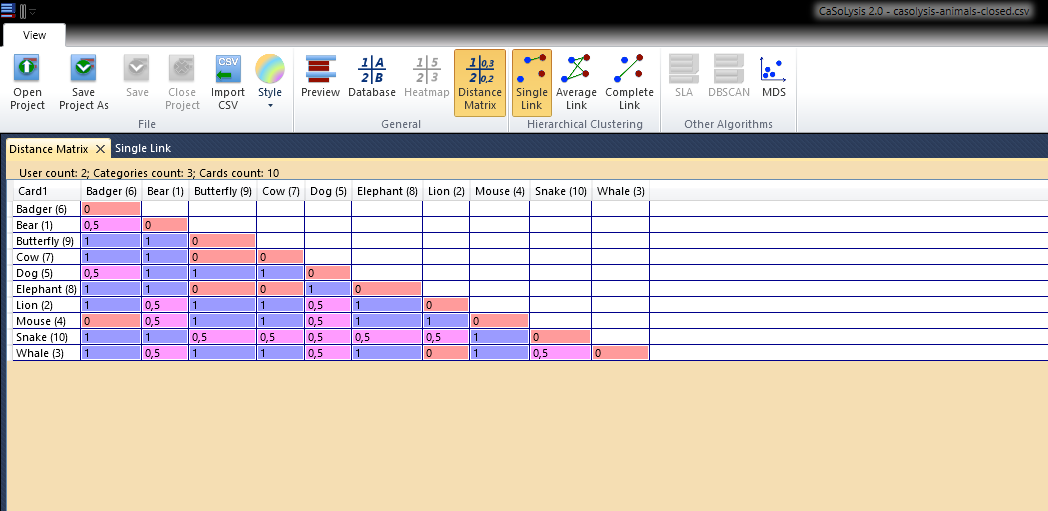
\includegraphics[keepaspectratio,width=\linewidth,height=\halfh]{images/casolysis-diagram-1.png}
\caption[Casolysis Distance Matrix] { This screenshot shows a distance
matrix over all cards that are used for analytics.
\imgcredit{Screenshot was captured by Christopher Oser using
\textcite{Casolysis}.} }
\label{fig:Casolysis2}
\end{figure}

\begin{figure}[tp] 
\centering
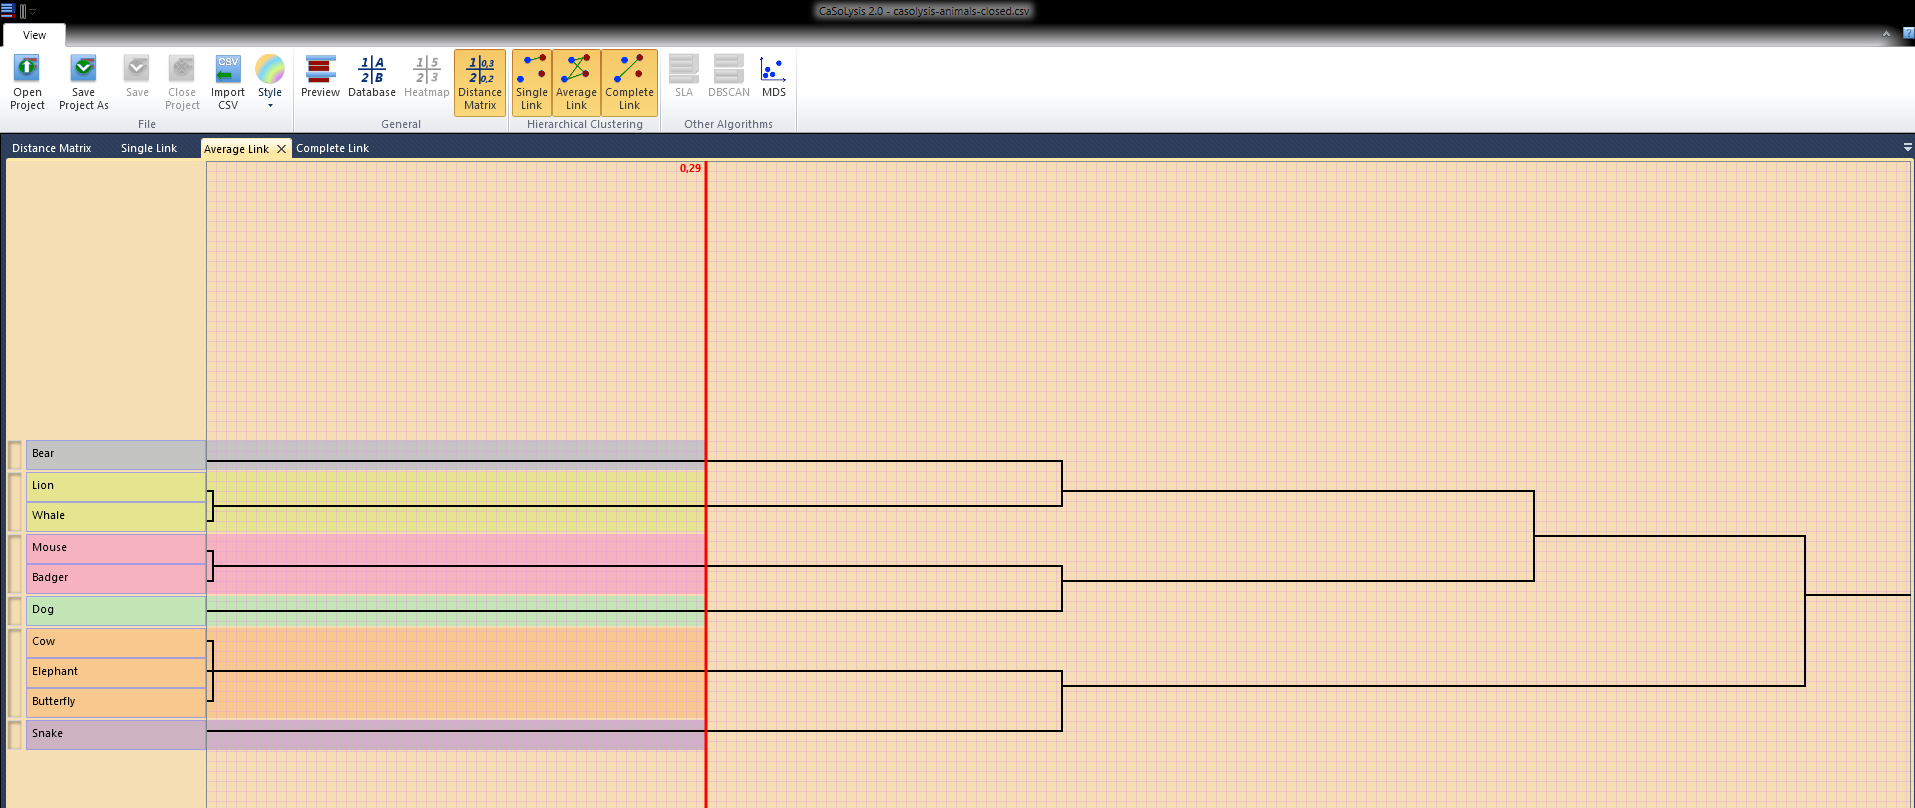
\includegraphics[keepaspectratio,width=\linewidth,height=\halfh]{images/casolysis-diagram-2.png}
\caption[Casolysis Dendrogram] { This screenshot shows a dendrogram 
for the average link of cards which is used for analytics.
\imgcredit{Screenshot was captured by Christopher Oser using
\textcite{Casolysis}.} }
\label{fig:Casolysis3}
\end{figure}

\begin{table}[tp]
\centering
\begin{tabularx}
{\linewidth}{|l|X|}
\hline \textbf{Feature/Characteristic} & \textbf{Availability in Casolysis} \\ 
\hline Card Sorting & None. Paper Cards or other tools needed. \\ 
\hline Card Limit & None. \\
\hline Participant Limit & None. \\
\hline Analytics & Analytics with 5 different types of visualizations
with different versions for some of them. \\ 
\hline Documentation & None. \\
\hline Business Model & Free. No longer under development \\
\hline Import formats & .csv\\ 
\hline Export formats & None. Screenshots of visualizations possibly. \\ 
\hline Sub-Categories & Yes, sub-categories are supported \\ 
\hline Playback of user-sessions & No. \\ 
\hline Data preparation & Very little - open/closed and sub-categories.
Everything else must be done manually. \\ 
\hline
\end{tabularx} 
\caption[Feature summary of Casolysis] 
{ 
This table summarizes all the features and characteristics of Casolysis
to provide an easy to read overview.
}
\label{tab:features-Casolysis}
\end{table}


\section{Summary \& Ratings}
All in all Casolysis seems to be a more modern \textcite{SynCaps},
minus the extensive data preparation options. Nevertheless it offers
more analytics and does so in a much simpler way. The visualizations
are easy to understand and frankly, quite pleasing to the eye.

Since its development has ended, there will be no added features in
the future and any bugs that might occur will not be fixed. So this
should be taken into account when considering Casolysis.

If the features are sufficient and you do not require card sorting
capabilities the tool seems to be a great fit. The only final drawback
being, that it is offline and needs Windows to be run.

For a quick overview and to make it easier to compare to other tools
in this paper, four ratings were agreed upon to represent the tool. The ratings can be
found in Table~\ref{tab:rating-Casolysis} and range from 0-5.


\begin{table}[tp] 
\centering 
\begin{tabularx}{\linewidth}{|X|X|X|X|X|}
\hline
Simplicity & Documentation & Features & Business Model & Average \\ 
\hline 
4 & 0 & 4 & 5 & 3.25 \\ 
\hline 
\end{tabularx} 
\caption[Ratings for Casolysis] {
Ratings for Casolysis including the average rating.
} 
\label{tab:rating-Casolysis}




\end{table}

\cleardoublepage
\chapter{TOOL}

\label{chap:tool}


TOOL INTRODUCTION.


\section{Business Model}

\section{Card Sorting}

\section{Analytics}

\section{Summary \& Ratings}

\cleardoublepage
\chapter{Concluding Remarks}

\label{chap:Concl}



At the end of your survey, give a clear recommendation
as to which approach or tool to use in which situation.





\cleardoublepage
% for now, switch to language english
% hack to force unix date for biblio, biblatex 3.11
\begin{otherlanguage}{english}
\printbibliography[heading=bibintoc]
\end{otherlanguage}


\end{document}

